%!TEX root = Constructive Alignment for Introductory Programming.tex

\chapter{Constructively Aligned Introductory Programming Curriculum} % (fold)
\label{cha:example_impl}

\graphicspath{{Figures/CAIntroProg/}}

\cref{cha:approach} proposed an approach to delivering constructively aligned introductory programming unit based upon the principles from \cref{cha:guiding_principles}. The proposed approach makes uses portfolio assessment, with an objects-later approach that divides the programming content across two introductory programming units. This chapter provides an example implementation of this approach, demonstrating how the principles from \cref{cha:guiding_principles} and the model from \cref{cha:approach} can be realised in a programming curriculum.

Sections of this chapter relate to the two introductory programming units: introductory programming, and object oriented programming. For each of these units the subsections are ordered to follow the processes from \cref{cha:approach}. First we outline the definition of the intended learning outcomes, and the construction of the assessment criteria. This is followed by examples of the various teaching and learning activities and resources developed in implementing this curriculum, and details of their delivery. Finally each section concludes with an overview of how the portfolios were assessed.

\acain{need to fix this next section}

\section{Paradigm Choice} % (fold)
\label{sec:paradigm_choice}

The second aspect of the overall strategy is to define an approach for selecting unit content. \sref{sec:principles_to_guide_what_we_should_cover} presented a number of principles related to what should be taught in introductory programming, with \pref{itm:paradigm} indicating that the overall strategy needs to be defined around a programming paradigm. This section addresses the question of which programming paradigms were selected for introductory programming in this work.

%
%  There is lots of work on objects vs not objects - do you review in Chapter 2?  Else need
% to do short review here??
%

Prior to conducting this research we have experienced introductory programming using both imperative-first and objects-first approaches. Our view mirrors those of \citet{Rist:1996} who reported on plans and cognitive schemas, the fundamental units of program design. In relating plans to objects, \citet{Rist:1996} indicated that objects were not different, they were more, as objects require additional overhead related to defining object\footnote{Object structures are typically defined using classes or similar mechanisms in languages such as Java} structures. Given this, units that take an objects-first approach will still need to have a significant focus on procedural aspects, as indicated by \citet{Robins:2003}. This reasoning was echoed in the ``back to basics'' approach from \citet{Reges:2006}.

\pref{itm:focus} indicates that in this work we aim to have a clear focus to build an appropriately deep knowledge. If, as \citet{Rist:1996} claimed, objects are ``more'' then our principles indicate that an objects-later approach should be taken. This is further supported by the 2013 Computer Science Curricula \cite{CSC2013}, which listed primarily imperative programming concepts in its section on Software Development Fundamentals.

An objects-later approach also matches the concept-based approach outlined in \cref{cha:guiding_principles}. \pref{itm:concepts} indicates a focus on programming concepts, which are built on top of previously covered concepts to enable students to explore the language, and programming in general. By starting with imperative programming the unit can start with fundamental concepts, and work up to the concept of objects.

\citet{Reges:2006} back to basics approach taught imperative programming concepts using the Java programming language. Java is an object oriented programming language, and so in effect this approach taught students how \emph{not} to use Java. While we will adopt the imperative programming focus, \pref{itm:authentic} indicates that we must select a programming language that was designed for this purpose. The language choice is discussed in \cref{cha:example_impl}.

%
% You can cite your own paper (TALE? ACE?) describing development of the units :-)
%

While objects would not appear in the first programming unit, their importance in students' education remained a focus. Rather than seeing programming as being delivered in a single stand alone unit, we designed a sequence of two units that worked closely together. The first covered structured procedural programming, focusing on aspects such as control flow. The second focused on object oriented programming, which can then use a model driven approach similar to the one reported in \citet{Bennedsen:2004} but without having to cover procedural programming aspects such as control flow.

Given its focus on fundamentals, an objects-later approach was used in the curriculum presented in this work. This aligns well with the principles in \cref{cha:guiding_principles} with its focus on depth over breadth, and its ability to match the proposed concept-based approach to introductory programming. Object oriented programming was then the content of a second programming unit. The alignment of these two units to the \emph{what} principles from \cref{cha:guiding_principles} is outlined in the following list.
\begin{enumerate}[noitemsep,nolistsep]
	\item The first programming unit, introductory programming, aligned with the principles in the following way:
	\begin{itemize}[noitemsep,nolistsep]
		\item Content selection was guided by the structured procedural programming paradigm.
		\item Focus will be on fundamental programming concepts, which included functions and procedures, variables, control flow, parameter passing, etcetera.
		\item The chosen programming language, or languages, must have been designed for procedural programming.
	\end{itemize}
	\item The second programming unit, object oriented programming, aligned with the principles in the following way:
	\begin{itemize}[noitemsep,nolistsep]
		\item Content selection was guided by the object oriented programming paradigm.
		\item Focus will be on object oriented programming concepts including abstraction, encapsulation, inheritance and polymorphism, etcetera.
		\item The chosen programming language, or languages, must have been designed for object oriented programming.
	\end{itemize}
\end{enumerate}




\section{Introductory Programming} % (fold)
\label{sec:introductory_programming}

\subsection{Aims for Introductory Programming} % (fold)
\label{ssub:intro:aims}

The aim of the introductory programming unit was to introduce students to programming and software development fundamentals. While focusing on developing depth in this area, the holistic nature of the portfolio assessment approach meant that programming is placed in the context of software development in general. As a result, this unit will touch on a number of areas not traditionally associated with introductory programming.

The following sections outline the definition of the intended learning outcomes, the construction of the assessment criteria and the development of the teaching and learning resources for the introductory programming unit.

% subsubsection aims (end)

\subsection{Defining Intended Learning Outcomes} % (fold)
\label{sec:intro:intended_learning_outcomes}

The first process in creating the introductory programming unit was to define appropriate intended learning outcomes. This process was influenced by a number of factors as described in \cref{cha:approach} (see \sref{sub:defining_intended_learning_outcomes}). These factors are discussed below, and are followed by a description of the unit's intended learning outcomes.

\subsubsection{Influencing Factors} % (fold)
\label{ssub:influencing_factors}

\fref{fig:defining_ilos} shows the specific factors that influenced the definition of the introductory programming unit. Three specific aspects will be discussed in the following sections: the overall strategy, accreditation requirements and industry requirements. The objects-later approach meant that this unit focused on procedural programming concepts. Accreditation requirements from the Australian Computer Society (ACS) focused the content on the wider role of software development in general. Whilst the model curriculum from the Association for Computing Machinery (ACM) and Institute for Electrical and Electronic Engineers (IEEE) provided guidance from an industry perspective.

\begin{figure}[htbp]
	\centering
	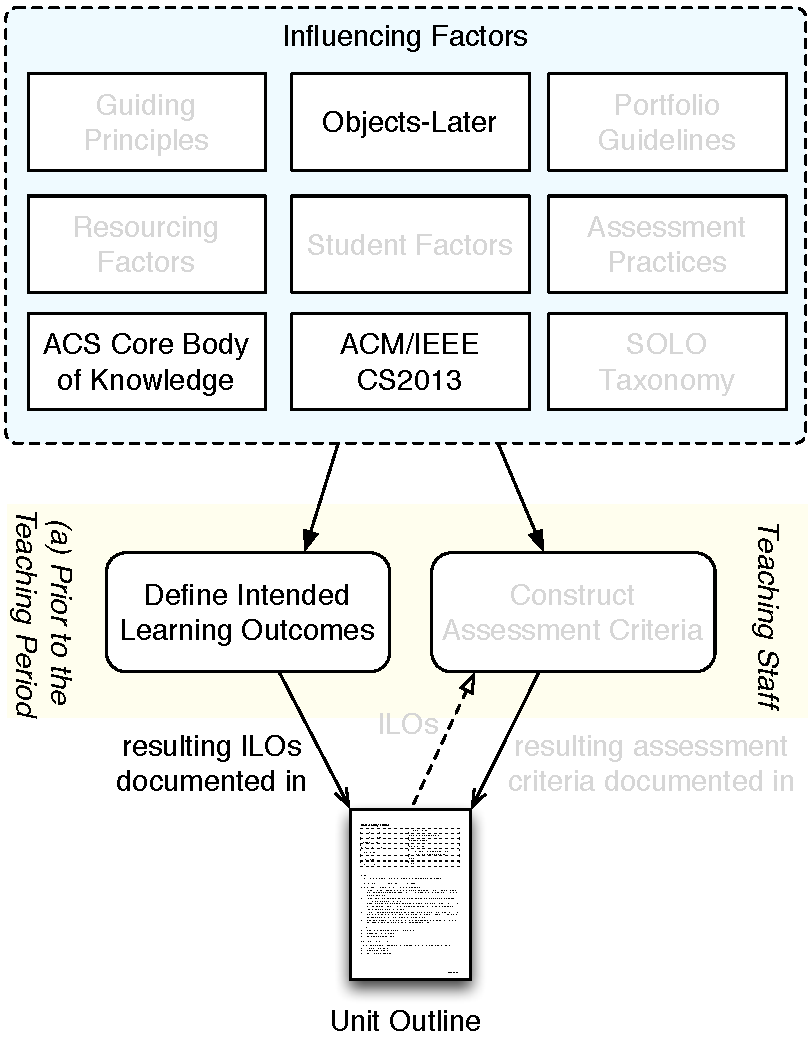
\includegraphics[width=0.7\textwidth]{ILOFactors}
	\caption{Factors that influenced the definition of the intended learning outcomes for introductory programming. \fref{fig:defining_ilos}}
	\label{fig:defining_ilos_intro}
\end{figure}

\paragraph{Objects-Later} % (fold)
\label{par:intro:objects_later}
The objects-later approach to this unit meant that it focused on structured and procedural programming concepts. The following list outlines the core concepts that were taught in this unit.

\begin{itemize}[noitemsep,nolistsep]
	\item Procedural programming abstractions:
	\begin{itemize}[noitemsep,nolistsep]
		\item Functional abstractions: functions and procedures
		\item Data abstractions: variables, constants, arrays and types
	\end{itemize}
	\item Structured programming principles:
	\begin{itemize}[noitemsep,nolistsep]
		\item Sequence, selection and repetition
		\item Control flow: pre-test and post-test loops, if and case
		\item Iteration over a collection
	\end{itemize}
	\item Program comprehension:
	\begin{itemize}[noitemsep,nolistsep]
		\item Memory layout: stack, heap and static memory
		\item Execution of control flow
		\item Parameter passing: pass-by-value and pass-by-reference
	\end{itemize}
\end{itemize}

% paragraph objects_later (end)

\paragraph{Accreditation Requirements} % (fold)
\label{par:accreditation_requirements}

The Australian Computer Society (ACS) documented the ICT profession and associated body of knowledge \cite{Gregor:2008}, which indicated graduates should develop both skills and knowledge as part of their undergraduate education. In the work, the skills component drew upon the Skills Framework for the Information Age (SFIA) while the knowledge area was divided into three aspects: a core body of knowledge, role specific knowledge and complementary knowledge. As a central role for a range of IT degrees, the introductory programming unit developed both student's skills and knowledge.

SFIA \cite{SFIA:2011} documented a range of IT skills across six categories. In terms of the SFIA, the Introductory Programming unit aimed to contribute to the development of \emph{programming and software development skill} from the \emph{Solution development and implementation} category. SFIA ranked each skill across seven levels of responsibility, ranging from \emph{follow} to \emph{set strategy, inspire and mobilise}. Introductory programming aimed to provide significant progress towards students attaining a Level 2, \emph{assist}, standard in this skill. To achieve this level of responsibility, students needed to demonstrate the ability to design, code, test, correct, and document simple programs, and indicated that students are able to assist with the development of a larger software solution.

The ACS divides the core body of knowledge into six areas: problem solving, professional knowledge, technology building, technology resources, service management and outcomes management. Introductory programming contributed toward the development of the problem solving, professional knowledge, technology building and technology resources as outlined in the following list:
\begin{itemize}[noitemsep,nolistsep]
	\item Problem solving:
	\begin{itemize}[noitemsep,nolistsep]
		\item Students used procedural programming abstractions, and were required to explain their various roles, properties and purpose. 
		\item Students followed methods and processes for designing and modelling procedural programming solutions.
	\end{itemize}
	\item Professional knowledge:
	\begin{itemize}[noitemsep,nolistsep]
		\item Students developed general computer competencies, including the use of compilers, shell scripting and basic BASH commands.
		\item Students read briefly about the history of computing, and the ICT discipline, providing a context for procedural programming and the structured programming principles.
		\item Professionalism, and the role of reflection and life-long learning in professional behaviour was instilled in students.
		\item Students performed self assessment of their competencies, and expertise, in applying procedural programming concepts. 
		\item The emphasis on demonstrating understanding enabled students to develop their written communication skills, including both technical and personal communications.
		\item Frequent interaction with staff aimed to help students development their interpersonal skills.
	\end{itemize}
	\item Technology building:
	\begin{itemize}[noitemsep,nolistsep]
		\item Students experienced many aspects of the software development lifecycle: undertaking simple analysis, design, implementation and testing processes.
		\item Students worked with iterative software development processes, building larger solutions across a number of iterations.
		\item The procedural programming topics listed above developed practical technology building skills.
		\item An understanding of the structured programming principles helped guide program construction and evaluation.
		\item Students used simple white box testing techniques to determine the success of their programs.
	\end{itemize}
	\item Technology resources:
	\begin{itemize}[noitemsep,nolistsep]
		\item Students developed a basic understanding of software systems, including the basics of software processes, memory layout and file systems.
	\end{itemize}
\end{itemize}

% paragraph accreditation_requirements (end)

\paragraph{Industry Requirements} % (fold)
\label{par:industry_requirements}

The Association for Computing Machinery (ACM) and IEEE Computer Society 2013 Computer Science Curriculum \cite{CSC2013} outlines a number of areas to be covered in a Computer Science curriculum. In terms of the ACM/IEEE model curriculum, the introductory programming unit primarily focused on \emph{Software Development Fundamentals}, but also integrated a number of other areas, as shown in the following list.

\begin{itemize}[noitemsep,nolistsep]
	\item Algorithms and Complexity:
	\begin{itemize}[noitemsep,nolistsep]
		\item \emph{Algorithmic Strategies}: students were introduced to divide-and-conquer, and the idea of recursive backtracking.
		\item \emph{Fundamental Data Structures and Algorithms}: all students programmed simple numeric algorithms, sequential search, and basic sorting.
	\end{itemize}

	\item Computational Science:
	\begin{itemize}[noitemsep,nolistsep]
		\item \emph{Processing}: fundamental programming concepts were covered in depth including algorithms,  implementing algorithms in code, and processes in the software development lifecycle.
	\end{itemize}

	\item Discrete Structures:
	\begin{itemize}[noitemsep,nolistsep]
		\item \emph{Basic Logic}: students used truth tables to learn to evaluate and construct boolean expressions.
	\end{itemize}
	
	\item Graphics and Visualisation:
	\begin{itemize}[noitemsep,nolistsep]
		\item \emph{Fundamental Concepts}: applications of computer graphics, double buffering and animation were covered to make programming more interactive.
		\item \emph{Geometric Modelling}: Optional tasks allowed students to explore procedurally generated models (fractals).
	\end{itemize}

	\item Human-Computer Interaction
	\begin{itemize}[noitemsep,nolistsep]
		\item \emph{Programming Interactive Systems}: students developed code to manage events and user interactions.
	\end{itemize}

	\item Programming Languages:
	\begin{itemize}[noitemsep,nolistsep]
		\item \emph{Basic Type Systems}: students explored the use of a range of basic types, along with the definition of custom enumerated and record types.
		\item \emph{Language Translation and Execution}: students are introduced to the topics of compilers and interpreters, as well as run-time layout of memory (call-stack, heap, static data), and manual memory management.
	\end{itemize}

	\item Software Development Fundamentals
	\begin{itemize}[noitemsep,nolistsep]
		\item \emph{Algorithms and Design}: students were introduced to the concept of algorithms, problem solving using divide-and-conquer, abstraction and program decomposition.
		\item \emph{Fundamental Programming Concepts}: students used programming language syntax, develop programs that contained statements, expressions, use variables, simple input and output operations, with conditional control flow, included functions, various parameter passing techniques, and were introduced to the concept of recursion.
		\item \emph{Fundamental Data Structures}: programs students implemented made use of arrays, record structures, strings and basic string processing, and students implemented a simple linked list.
		\item \emph{Development Methods}: program comprehension was central to the unit, with basic details of program correctness being introduced. Students were also required to use basic refactoring techniques to restructure code, and program tracing was covered as a debugging technique.
	\end{itemize}

	\item Software Engineering
	\begin{itemize}[noitemsep,nolistsep]
		\item \emph{Software Processes}: students used an iterative software development process model, and were introduced to the phases of the software development lifecycle. 
		\item \emph{Software Design}: students were introduced to the principles of the structured design paradigm, and used these principles in the design and development of the programs they created.
		\item \emph{Software Construction}: coding standards, and defensive coding practices were introduced to students.
	\end{itemize}

	\item Social Issues and Professional Practice:
	\begin{itemize}[noitemsep,nolistsep]
		\item \emph{Professional Ethics}: students develop skills in professional practice including self assessment, reflective practice, computer fluency, and general approach to life-long learning.
		\item \emph{Professional Communication}: to demonstrate their understanding students were required to read, understand and communicate technical material using clear language and visual mediums.
	\end{itemize}

\end{itemize}

% paragraph industry_requirements (end)

% subsubsection influencing_factors (end)

\subsubsection{Intended Learning Outcomes} % (fold)
\label{ssub:intro_intended_learning_outcomes}

All of the factors listed above, and those from \cref{cha:approach}, guided the definition of the intended learning outcomes for introductory programming. Given the wide range of skills and knowledge mentioned above, the challenge was to ensure that this could be expressed in a small number of intended learning outcomes. This task was assisted by the use of the SOLO taxonomy, and recognising that the SOLO level of each outcome indicated that earlier levels must already have been achieved.

The final statement of the intended learning outcomes for introductory programming are listed below, with the verbs from the SOLO taxonomy highlighted.
\begin{enumerate}[noitemsep,nolistsep]
	\item \textbf{Apply} code reading and debugging techniques to \textbf{analyse}, \textbf{interpret}, and \textbf{describe} the purpose of program code, and \textbf{locate} within this code errors in syntax, logic, and/or good practice.
	\item \textbf{Describe} the principles of structured programming, \textbf{relate} these to the syntactical elements of the programming language used, and the way programs are developed using this language.
	\item \textbf{Construct} small programs, using the programming languages covered that include the use of arrays, functions and procedures, parameter passing with pass-by-value and pass-by-reference, custom data types, and pointers.
	\item \textbf{Use} modular and functional decomposition to break problems down functionally, \textbf{represent} the resulting structures diagrammatically, and \textbf{implement} the structure in code as functions and procedures.
\end{enumerate}

Introductory programming used a procedures-first approach, and focused on the structured programming principles of organising code using \emph{sequence}, \emph{selection} and \emph{repetition}. Students learnt to use functional and modular decomposition to break problems down, and implement solutions using functions and procedures. Data was managed using arrays and custom data types. Pointers and memory management were introduced. Various forms of parameter passing were covered, including pass-by-value and pass-by-reference. Weaved through this was an iterative development process, a focus on writing clear and legible code, and other good programming practices. In addition to writing code, students learnt to read code for the debugging purposes, and to demonstrate their ability to interpret other peoples code.

Each outcome aims to engage students in activities that will help them achieve a \emph{relational} level of understanding. The verbs \emph{analyse}, \emph{apply}, \emph{construct}, \emph{implement}, \emph{interpret} and \emph{use} represent activities in which students will need to use cognitive activities that will help them achieve a relational level of understanding. The multistructural \emph{describe} verb and the unistructural \emph{locate} verb are also used, but as a supporting activity for a higher level verb, such as with describe and relate.

Many of the factors listed above are not directly stated as intended learning outcomes, but were an important part of the delivery of the unit. The decision to not include additional factors in the intended learning outcomes was a result of ensuring a clear focus within the recommended number of items; being between four and six. The remaining factors were addressed by the means through which students achieved these intended learning outcomes. This included professional communication, software engineering methods and graphics and visualisation.

\paragraph{Professional Communication} % (fold)
\label{par:professional_communication}

Traditionally, programming units focused on assessing code outcomes. Assuming that if students could produce the code, then they understood it. Others, such as \citet{Lister:2004}, have extended this to include small code reading and tracing tasks in order to expand on the assessment of student's understanding of code. With this introductory programming unit this is taken further, with the students needing to write about the associated principles and to describe code. This expanded assessment had the dual benefit of engaging higher levels of cognitive activity, while also helping students to develop their professional communication skills.

Each of the intended learning outcomes requires students to communicate their understanding. For example, in meeting the first outcome students needed to demonstrate the ability to interpret supplied code, and to communicate its purpose and any issues in logic or the application of recommended good practice. While not a direct focus of the assessment, communication skills play an enabling role in achieving this, and students were provided with support and encouragement in developing their communication skills alongside their technical skills.

% paragraph professional_communication (end)
 
\paragraph{Software Engineering Methods} % (fold)
\label{par:software_engineering_methods}

While typically the focus of later software engineering units, the software development lifecycle and iterative development methods were embedded within the unit. Students engaged in the development of software throughout the unit: analysing, designing, developing and testing software became a means for them to achieve these outcomes. Students experienced the software development lifecycle first hand, without needing it to be stated in the unit's intended learning outcomes.

Larger programs in the unit were broken down into a number of iterations, and students build these solutions by performing these iterations. Once again, this enabled them to experience software development methods without these methods being explicitly included in the assessed outcomes.

Together, both of these aspects were related to the more general concept of \emph{problem decomposition}. The idea of approaching a solution through discrete iterations provided an example of decomposing a problem into smaller steps. Similarly, the idea of breaking each of these steps into more manageable processes was used to explain both the idea of decomposition and the software development lifecycle. 

% paragraph software_engineering_methods (end)

\paragraph{Graphics and Visualisation} % (fold)
\label{par:graphics_and_visualisation}

Identifying appropriate applications for student to develop is a common problem with teaching introductory programming. In teaching introductory programming it was decided to focus on having students program small computer games. The research literature related to the use of games indicates that this is popular with students, and helps motivate them to spend time on the task, as shown in the following list.

\begin{itemize}[noitemsep,nolistsep]
	\item \citet{Roberts:1995} used a graphical library in teaching introductory programming and reported that it enhanced student interest and reinforced essential programming concepts.

	\item \citet{Feldgen:2004} reported their highest class attendance for the unit after shifting to using games, with improvements in pass rates and student retention.

	\item The greenfoot environment, introduced in \citet{Kulling:2005}, was created to help introduce high school students to object oriented programming.

	\item \cite{Rajaravivarma:2005} used text based and numeric games as a domain for introductory programming and indicated the approach created a ``passion to want to do more''.

	\item \citet{Bayliss:2006} discussed the use of games in a summer distance unit introducing students to programming and concepts in computer science. The work reported that a large percentage of students enjoyed learning introductory programming concepts in the context of games.

	\item Results from \citet{Cliburn:2006} suggested that for a large majority of students games had provided psychological motivation and had increased unit enjoyment.

	\item \citet{Leutenegger:2007} reported that games had improved student understanding of all basic topics examined.

	\item \citet{Sung:2009} provided some guidelines on incorporating games into introductory programming. This indicated an need to ensure tools are freely available, that core concepts need to remain the focus, and that games should aim to be gender and expertise neutral.

	\item \citet{Sung:2011} introduced game-themed programming assignments to help teaching staff make the transition to game based introductory programming.

\end{itemize}

The use of games as a context for software development requires students to gain some familiarity with fundamental concepts related to graphics and animation. The interactive nature of these games also introduces students to the concept of programming in response to user input events.

% paragraph graphics_and_visualisation (end)

\subsection{Constructing Assessment Criteria} % (fold)
\label{sub:intro_constructing_assessment_criteria}

The construction of the assessment criteria happened alongside the definition of the intended learning outcomes. The goal here, as stated in \cref{cha:approach}, was to create clearly distinct grades where each grade required students to demonstrate a better understanding of software development. 

\fref{fig:assessment_criteria} shows the assessment criteria for the introductory programming unit. Each of the grades uses the levels discussed in \cref{cha:approach}. For \emph{Pass} and \emph{Credit} students completed the set exercises, which were only signed off through student interaction with staff. \emph{Distinction} required the implementation of a program of the student's own creation, which \emph{High Distinction} required a small research project.

\begin{figure}[htbp]
	\centering
	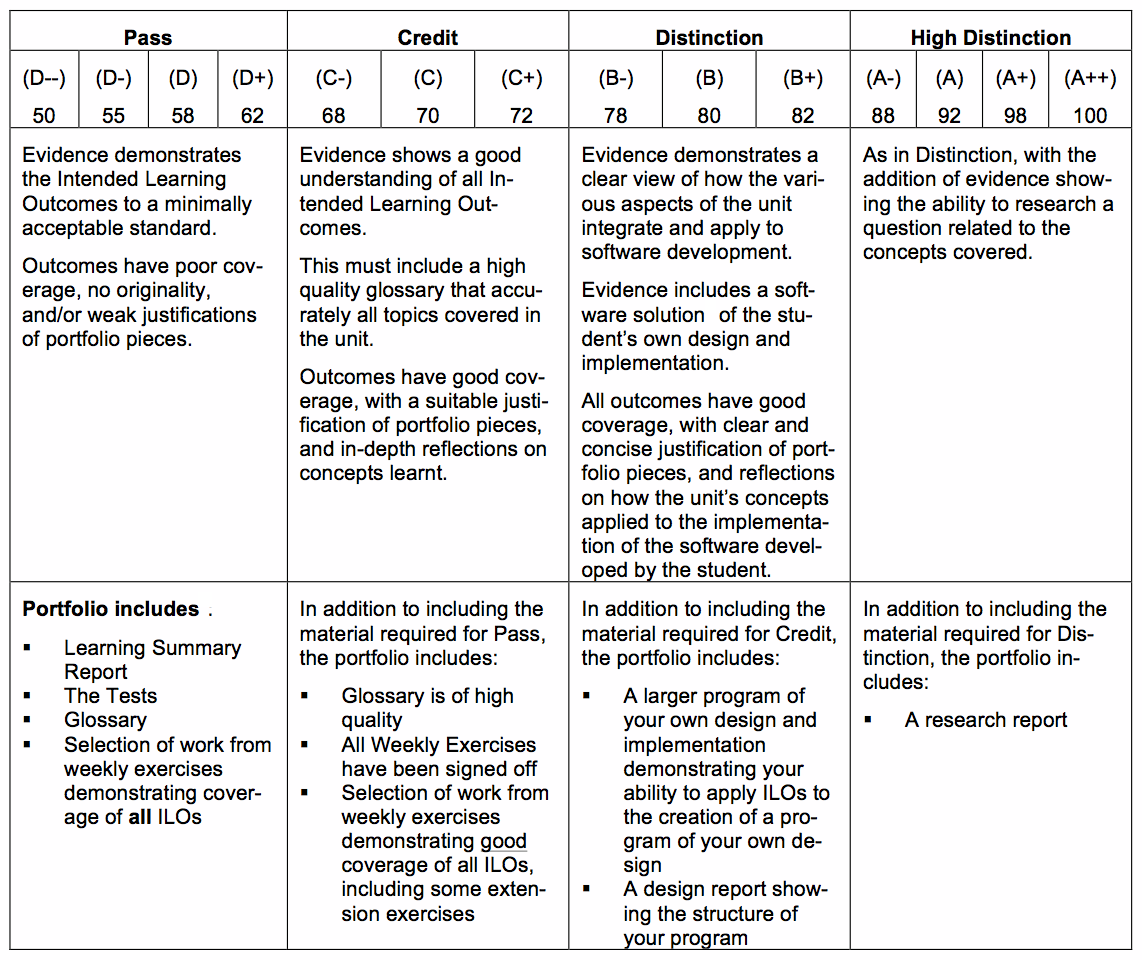
\includegraphics[width=\textwidth]{AssessmentCriteria}
	\caption{The assessment criteria from the Unit Outline of the introductory programming unit.}
	\label{fig:assessment_criteria}
\end{figure}

To receive at least a Pass grade, students needed to satisfactorily complete three hurdle tests as well as including a number of pieces of work that demonstrated they had met all of the intended learning outcomes. These pieces of work needed to work from the weekly tasks, but did not need to have been signed off by teaching staff. 

The \emph{Credit} grade required students to meet all pass requirements, and to have succeeded in getting all tasks signed off. This ensured we were happy they had completed the work themselves and providing them with incentives to engage in the formative feedback process. Their explanation of programming concepts and abstractions, in their Glossaries, was the main item to distinguish between Pass and Credit in terms of depth of understanding. In this regard, the student's glossary needed to demonstrate good coverage of all outcomes for the student to be eligible for a Credit grade.

\emph{Distinction} built on top of the Credit requirements and required students to create a program of their own design. This could be any program the student was interested in creating, as long as it demonstrated good coverage of all of the unit's intended learning outcomes. In effect, this meant that students needed to create a program that contained a number of functions and procedures, used arrays and record types, and was of sufficient size and complexity. Most students who received this grade had implemented a game of some kind, many emulating classic arcade games such as asteroids, pong, frogger or space invaders.

\emph{High Distinction} required students to engage in the creation of a short research report, in addition to having met the Distinction grade requirements. Each student aiming to achieve this grade worked together with staff to define a topic they could examine, and then the student carried out data collection, analysis and reporting tasks. As an introductory programming unit, this research was limited to examining simple tasks such as algorithm efficiency, different techniques to perform a task, or comparing performance aspects of different code. Students were encouraged to think deeply about their results, and to document their outcomes clearly.

% subsection constructing_assessment_criteria (end)

\subsection{Developing Teaching and Learning Activities} % (fold)
\label{sub:intro_developing_teaching_and_learning_activities}

Allocated classes for the introductory programming unit included a two hour lecture, and a two hour laboratory class each week, over a thirteen week teaching period. All classes were designed with the goal of actively engaging students. A typical lecture included a short presentation using ``Beyond Bullet Points'' style lecture slides \cite{Atkinson:2007}, an interactive programming demonstration and group activities. In the laboratory sessions, students were involved in code reading activities, guided programming tasks and practical hands-on exercises.

The teaching period consisted of thirteen weeks, twelve of which were teaching weeks, and a single week semester break. Topics for the twelve lectures are shown in the following list. In weeks one to six students explored these concepts using a modern version of the Pascal programming language \cite{Wirth:1971,FPC:2011}. In week 7 students were introduced to the C programming language \cite{Ritchie:1978}, which was used for the remainder of the semester. 

\begin{enumerate}[noitemsep,nolistsep]
  \item Programs, Procedure, Compiling and Syntax
  \item User Input and Working with Data
  \item Control Flow: Branches and Loops
  \item Procedural and Structured Programming
  \item Arrays
  \item Custom Data Types and Pointers
  \item Learning a New Language
  \item Programming in C
  \item File Input and Output
  \item Dynamic Memory Management
  \item Recursion and Backtracking
  \item Review and Future Studies
\end{enumerate}

\acain{lots cut from here}

% lecture stuff removed from later... After switching programming language the situation changed, and the concepts were now being reinforced. In these lectures the presentations were delivered in their entirety before the interactive sessions. This helped reinforce the idea that the concepts were the same, all that had changed was how these concepts are expressed in code. Progressing through the concepts quickly promoted their value, and reassured students that the concepts they had already learnt still applied.

% It is important to note that at no point in either the presentation or the interaction sessions was the syntax fully described. Instead, students were equipped with knowledge of the concepts and the skills to learn the language themselves. Language details were of secondary importance, and resources containing the relevant details were made available for them to explore as they needed.

% Extension tasks were provided to push students, and to encourage them to think about starting work on the custom and research projects necessary to receive higher grades. These tasks were related to each weeks concepts, but were loosely defined, requiring students to take greater responsibility for the analysis and design of the solution.

% Each week's laboratory class consisted of a number of activities. At the start of the class the teaching staff returned the feedback from the previous week's core exercises, but delayed discussing feedback with students until after working through the exercises. Students where then guided through the week's laboratory exercises, and the core exercises were discussed. Students spent the remaining laboratory time on the week's core exercises. During this time the teaching staff visited each student individually to discuss their progress, and to mark their work as signed off.



The core exercises also had students documenting their understanding of the core concepts each week in a glossary. The glossary recorded details on the following aspects of the unit:
\begin{itemize}[noitemsep, nolistsep]
	\item Core concepts:
	\begin{itemize}[noitemsep, nolistsep]
		\item Control flow
		\item Structured programming principles
		\item Functional and modular decomposition
		\item Good programming practices
	\end{itemize}
	\item Programming terminology:
	\begin{itemize}[noitemsep, nolistsep]
		\item Statements
		\item Expressions
		\item Identifiers
		\item Parameters, local variables and global variables
	\end{itemize}
	\item Programming abstractions:
	\begin{itemize}[noitemsep, nolistsep]
		\item Programs
		\item Functions and Procedures
		\item Constants and Variables
		\item Arrays
		\item Records and Enumerations
		\item Pointers
	\end{itemize}
	\item Statements:
	\begin{itemize}[noitemsep, nolistsep]
		\item Function and procedure calls
		\item Assignment statements
		\item If and case statements
		\item While and repeat/do..while loops
		\item For loops
	\end{itemize}
\end{itemize}

\begin{figure}[p]
	\centering
	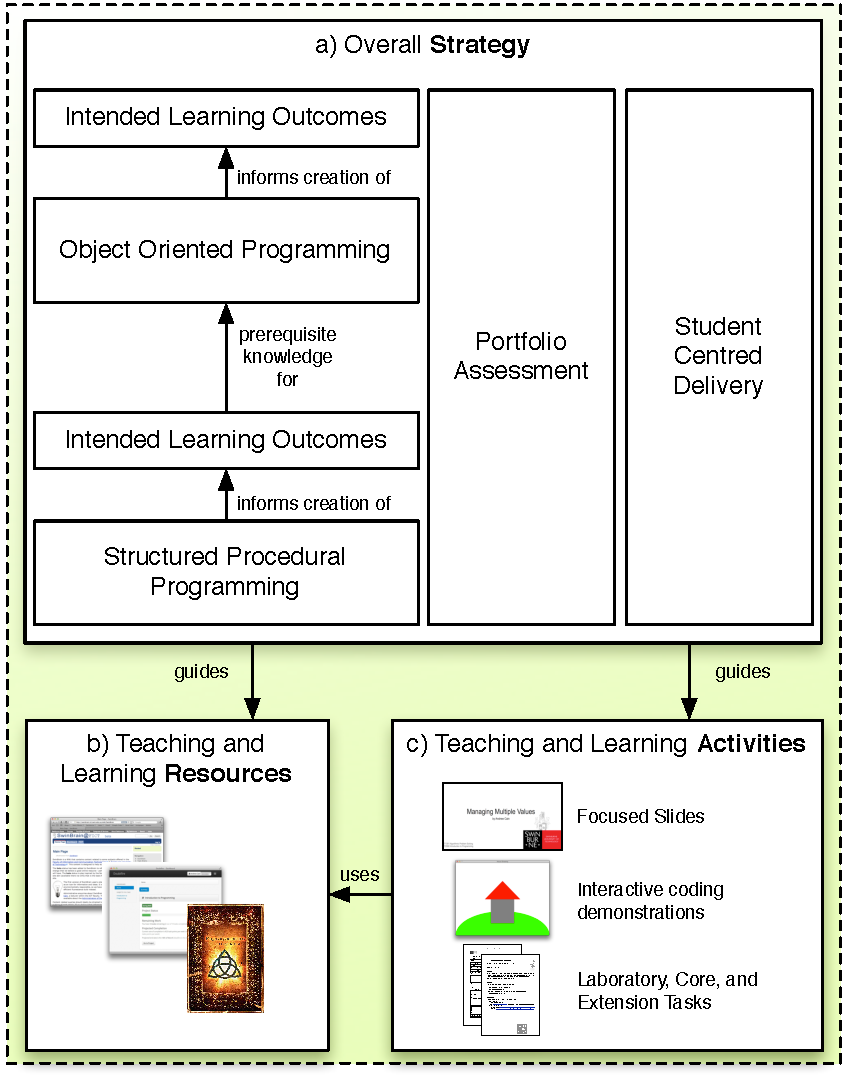
\includegraphics[width=\textwidth]{OverallStrategy}
	\caption{An updated version of \fref{fig:strategy} showing the selected assessment approach, and the programming paradigms that will form the approach for selecting content.}
	\label{fig:overall_strategy}
\end{figure}


\subsubsection{Procedures First Topic Sequence} % (fold)
\label{ssub:procedures_first_topic_sequence}

The order of topics was guided by the principles from \cref{cha:guiding_principles}. The main objective being to enable each week's topic to build upon earlier topics, while providing a consistent set of abstractions for students to work with.

This was achieved using a procedures-first approach, an approach which \citet{Pattis:1990} indicated was popular in textbooks prior to the current objects-first range. This approach has students program their own procedures from week 1. The following list indicates the concepts, programming abstractions and statements introduced each week.

\begin{enumerate}[noitemsep,nolistsep]
  \item Programs, Procedure, Compiling and Syntax
  \begin{itemize}[noitemsep,nolistsep]
  	\item \textbf{Sequence}: the focus of this week was on programs and procedures as a \emph{sequence} of instructions that get the computer to perform a task.
  	\item \textbf{Syntax Rules}: students learnt to use visual ``railroad'' diagrams \cite{Braz:1990} to understand programming language syntax.
  	\item \textbf{Program}: students created small programs that contained a sequence of procedure calls, with all values being hard coded.
  	\item \textbf{Procedure}: students developed a small number of procedures, each with a defined task that contributed to the overall program.
  \end{itemize}
  \item User Input and Working with Data
  \begin{itemize}[noitemsep,nolistsep]
  	\item \textbf{Data}: The central idea of this week was \emph{data}, the idea that values can be stored and calculated.
  	\item \textbf{Variables}: students created local variables, global variables and parameters.
  	\item \textbf{Constants}: students declared constants.
  	\item \textbf{Functions}: students used functions in the laboratory and core exercises, and developed their own in the extension tasks.
  	\item \textbf{Assignment Statements}: students used assignment statements to store values in variables. 
  \end{itemize}
  \item Control Flow: Branches and Loops
  \begin{itemize}[noitemsep,nolistsep]
  	\item \textbf{Control Flow}: the ideas of sequence, selection and repetition were central to this week.
  	\item \textbf{Selection}: students used \textbf{if statements} and  \textbf{case statements} to implement branching in their control flow.
  	\item \textbf{Repetition}: students repeated code using \textbf{while loops} and \textbf{repeat loops}.
  \end{itemize}
  \item Procedural and Structured Programming
  \begin{itemize}[noitemsep,nolistsep]
  	\item \textbf{Functional and Modular Decomposition}: the idea of solving problems using divide-and-conquer was the main theme of this week.
  	\item \textbf{Software Development Lifecycle}: the basic steps of the software development lifecycle were discussed.
  	\item \textbf{Iterative Development}: the idea of iteratively working toward a solution was discussed.
  	\item \textbf{Structured Programming}: the structured nature of a functions/procedures code was discussed, illustrating how these steps can be broken down into blocks performing sequence, selection or repetition.
  	\item No new programming abstractions or statements were introduced in this week.
  \end{itemize}
  \item Arrays
  \begin{itemize}[noitemsep,nolistsep]
  	\item \textbf{Arrays}: students started to use arrays to store multiple values in their programs.
  	\item \textbf{For loops}: the for loop was introduced as a convenient means of looping through the contents of an array, allowing the code to easily apply a set of operations on each element in the array.
  \end{itemize}
  \item Custom Data Types and Pointers
  \begin{itemize}[noitemsep,nolistsep]
  	\item \textbf{Types}: custom types and the role of types in a programming languages were discussed.
  	\item \textbf{Records}: students developed their own custom record types to model entities associated with their programs.
  	\item \textbf{Enumerations}: students use of enumerations as a means of creating a type to represent a list of options.
  	\item \textbf{Pointers}: pointers were used to create relationships between values, and to illuminate how pass-by-reference worked internally.
  \end{itemize}
  \item Learning a New Language
  \begin{itemize}[noitemsep,nolistsep]
  	\item \textbf{Language Syntax}: ways to approach a new programming language were discussed, and students used a new language to recreate previously developed programs.
  \end{itemize}
  \item Programming in C
  \begin{itemize}[noitemsep,nolistsep]
  	\item No new programming concepts or abstractions were presented in this week. Instead the week was used to consolidate knowledge of the new language, and to develop a wider range of programs using the previously presented concepts.
  \end{itemize}
  \item File Input and Output
  \begin{itemize}[noitemsep,nolistsep]
  	\item \textbf{File Input and Output}: the idea of persisting data was presented, and students learnt to save data to a file and read it back. 
  \end{itemize}

  \item Dynamic Memory Management
  \begin{itemize}[noitemsep,nolistsep]
  	\item \textbf{Stack and Heap}: specifics related to memory layout were discussed, including the limitations of the stack.
  	\item \textbf{Dynamic Memory Allocation}: students used memory allocation functions to allocate memory from the Heap, and used pointers to work with the newly allocated space.
  \end{itemize}

  \item Recursion and Backtracking
  \begin{itemize}[noitemsep,nolistsep]
  	\item \textbf{Recursion}: students developed simple recursive solutions for problems like the Fibonacci sequence and the Towers of Hanoi.
  	\item \textbf{Backtracking}: the idea that a recursive solution can backtrack to search alternative paths was discussed, and extension tasks introduced backtracking to solve Sudoku and the Eight Queens puzzle.
  \end{itemize}

  \item Review and Future Studies
  \begin{itemize}[noitemsep,nolistsep]
  	\item This week did not introduce any new programming concepts or abstractions, instead it was used to review everything that had been covered and to discuss future programming units.
  \end{itemize}
\end{enumerate}

\citet{Pattis:1990,Pattis:1993} indicated that the main challenge with the procedures first approach was that students did not have anything meaningful to program in their procedures prior to introducing control flow. \citet{Pattis:1993} reported that the majority of procedures-first texts had moved control flow prior to procedure declarations in response to this issue. We took an alternative approach, and introduced students to a game development framework in week one. This framework provided a range of useful procedures that students could call, and thereby addressed the issues that Pattis had raised. Details of this game development framework are presented in \cref{cha:supporting}.

The following list outlines the focus of each week's tasks.
\begin{enumerate}[noitemsep,nolistsep]
  \item Programs, Procedure, Compiling and Syntax
  \begin{itemize}[noitemsep,nolistsep]
  	\item \textbf{House Drawing}: students created a procedure to draw a house at a fixed location on the screen.
  	\item \textbf{Knock Knock}: students created a number of procedures to show images and play sound effects necessary to display a knock knock joke.
  	\item \textbf{Custom Splash}: extensions encouraged students to develop a procedure to show their own splash screen.
  \end{itemize}
  \item User Input and Working with Data
  \begin{itemize}[noitemsep,nolistsep]
  	\item \textbf{House Drawing}: the fixed house was redeveloped to make use of parameters and local variables, allowing its position to be changed.
  	\item \textbf{Bike Drawing}: students developed a procedure to draw a fixed size bike, using parameters for the bike's location and colour.
  \end{itemize}
  \item Control Flow: Branches and Loops
  \begin{itemize}[noitemsep,nolistsep]
  	\item \textbf{Lots of Bikes}: students created a custom screen saver like program that drew thousands of bikes to the screen.
  	\item \textbf{Circle drawing}: students developed a program in which they could move a circle around the screen, switching it between outlined and filled, or clicking it to make it jump to a random position.
  \end{itemize}
  \item Procedural and Structured Programming
  \begin{itemize}[noitemsep,nolistsep]
  	\item \textbf{User input functions}: students created functions to read strings, integers, doubles, and ranges of values (between a minimum and maximum) from the user. These build on top of each other to demonstrate the power of functional decomposition.
  	\item \textbf{Arcade game}: students were encouraged to develop a simple clicking arcade game using the concepts already covered.
  \end{itemize}
  \item Arrays
  \begin{itemize}[noitemsep,nolistsep]
  	\item \textbf{Statistics}: students developed a program that read in a number of values from the user and then calculated a number of statistics. This included median, which required the values in the array to be sorted.
  \end{itemize}
  \item Custom Data Types and Pointers
  \begin{itemize}[noitemsep,nolistsep]
  	\item \textbf{Address Book}: a simple address book, with links to friends was developed to demonstrate records and pointers.
  	\item \textbf{Pop Game}: provided a larger, multiple iteration, project in which students developed a simple arcade style game. The game involved popping different kinds of shapes, with rounds of ten shapes each of random sizes and colours.
  \end{itemize}
  \item Learning a New Language
  \begin{itemize}[noitemsep,nolistsep]
  	\item \textbf{User input functions}: students redeveloped the user input functions using the new programming language. 
  \end{itemize}
  \item Programming in C
  \begin{itemize}[noitemsep,nolistsep]
  	\item \textbf{Statistics} was reimplemented in the new programming language.
  \end{itemize}
  \item File Input and Output
  \begin{itemize}[noitemsep,nolistsep]
  	\item \textbf{Address Book}: students reimplemented the address book in C, and added the ability to save it to file, and load it from file. 
  \end{itemize}

  \item Dynamic Memory Management
  \begin{itemize}[noitemsep,nolistsep]
  	\item \textbf{Address Book}: dynamic memory management was used to allow for a variable number of contacts in the address book.
  	\item \textbf{Maze Game}: extension tasks had the students develop a network of rooms connected using pointers.
  \end{itemize}

  \item Recursion and Backtracking
  \begin{itemize}[noitemsep,nolistsep]
  	\item \textbf{Recursive Programs}: extension tasks had students develop recursive functions.
  	\item \textbf{Linked List}: extension tasks demonstrated how to use pointers and records/structures to create a linked list.
  \end{itemize}

  \item Review and Future Studies
  \begin{itemize}[noitemsep,nolistsep]
  	\item There was no lab exercises this week, the lab was used to help students complete any outstanding tasks.
  \end{itemize}
\end{enumerate}

% subsubsection procedures_first_topic_sequence (end)

\subsubsection{Programming Language Choice} % (fold)
\label{ssub:programming_language_choice}

Introductory programming aimed to teaching students to \emph{program}, not the details of a programming language. We did not aim to develop students' expertise in one programming language, but to equip them with the knowledge and skills to become experts in \textbf{any} imperative programming language.

Whenever discussing introductory programming it is always interesting to note how quickly people jump to the question of language. In the delivery of this unit the programming language was always a secondary concern, an enabling feature not an aspect of great importance. The language choice was made based on its ability to support the following requirements:
\begin{itemize}[noitemsep,nolistsep]
	\item \textbf{Explicit} \emph{over} implicit
	\begin{itemize}[noitemsep,nolistsep]
		\item Require explicit variable declaration, with clear indication of the variable's type.
		\item Strongly typed, avoiding implicit type conversions.
	\end{itemize}

	\item \textbf{Procedural programming abstractions} \emph{over} support for other paradigms.
	\begin{itemize}[noitemsep,nolistsep]
		\item Functions and procedures.
		\item Pass-by-value and pass-by-reference.
		\item Arrays, constants and variables.
		\item Declaration of custom types including enumerations and record structures.
		\item Pointers and dynamic memory management.
	\end{itemize}
\end{itemize}

\begin{table}
	\renewcommand{\arraystretch}{1.6}
	\centering
	\caption{Comparison of programming languages for the introductory programming unit.}
 	\label{tbl:language_comparison}

    \begin{tabular}{l|c|c|c|c|c|c}
    ~                                   & C   & C++ & C\#     & Java & Pascal & Python \\ \hline
    Explicit Variables                  & Yes & Yes & Yes     & Yes  & Yes    & ~      \\
    Strongly Typed                      & ~   & ~   & Yes     & Yes  & Yes    & Yes    \\
    Functions and procedures            & Yes & Yes & Partial & ~    & Yes    & Yes    \\
    Parameter passing options & ~   & Yes & Yes     & ~    & Yes    & ~     \\
    Data abstractions     & Yes & Yes & Yes     & Yes  & Yes    & Yes    \\
    Records and enumerations  & Yes & Yes & Yes     & ~    & Yes    & ~      \\
    Pointers                            & Yes & Yes & Partial & ~    & Yes    & ~      \\
    Explicit memory management & Yes & Yes & ~ & ~    & Yes    & ~      \\
    Used by staff     & Yes & Yes & Yes     & Yes  & Yes    & Yes    \\
    \end{tabular}
\end{table}

\tref{tbl:language_comparison} lists the languages considered for the introductory programming unit. Pascal met all of the requirements, with C++ and C\# satisfied most. C\# was designed for object oriented programming, and therefore using it for procedural programming was against \pref{itm:authentic} which indicated we would only use languages as they were designed to be used. 

The choice between C++ and Pascal was more challenging. C++ had the advantage of being widely used, and the popularity of the C-style syntax would mean that it apply more directly to other languages. However, the C++ language itself is cryptic and would be more challenging for students to master on their own. Pascal, on the other hand, was seen as having a more ``beginner friendly'' syntax. Pascal had also been used by \citet{Becker:2002}, who stated that it had enabled them to focus less on the syntax, as compared to C++.

Rather than choosing \emph{either} language it was decided to take advantage of the strength of both languages, and it was decided to use \emph{both}. Students would be able to focus more on the concepts using Pascal's more friendly syntax over the first few weeks of the semester. Once all the concepts were covered the language could be switched and students could explore the procedural aspects of C++, getting a start with a C-style syntax.

The focus on teaching students to ``understanding syntax'' from week one supported, and was supported by, the change of language. Students had been exposed to programming language syntax using the visual ``railroad'' diagram syntax notation \cite{Braz:1990}, and had used this to learning Pascal over the first weeks of the unit. After the switch to C++, students could reinforce these same skills by applying them to learn a second programming language. This approach aimed to encourage students to focus on the concepts, which would then enable them to more quickly learning the new language.

% subsubsection programming_language_choice (end)

% subsection developing_teaching_and_learning_activities (end)


\subsection{Delivering the Unit} % (fold)
\label{sub:delivering_the_unit}

Delivery of the unit followed the process outlined in \cref{cha:approach}, and used the activities outlined in the previous section. Each week the lecture presented the relevant concepts, with demonstrations introducing students to the syntax. The laboratory sessions helped students prepare for the core tasks, which they completed after each class. The completed core and extension tasks were submitted for formative feedback at the start of the next weeks lecture and the process repeated across each week of the teaching period.

A Programming Help Desk was also made available to students during the week. This was staffed by later year students, and teaching staff from the unit. Students could drop in to the help desk to help clarify any issues they had with the concepts of programming language syntax.

The unit made heavy use of the university's online learning management system to provide additional support for students outside of scheduled class times. The use of the discussion board was actively encouraged, and questions were promptly answered by teaching staff, and in some cases by fellow students. 

% subsection delivering_the_unit (end)


\subsection{Assessing Student Portfolios} % (fold)
\label{sub:assessing_student_portfolios}

At the end of the teaching period student portfolios were assessed using the process shown in \fref{fig:assessment_process}. This illustration had been included in the unit outline, to help communicate the assessment approach to the students.This portfolio assessment involved the following steps:

\begin{enumerate}[noitemsep,nolistsep]
	\item Determine the grade from the self assessment, cross referenced with data collected from the student during the teaching period.
	\item Initially assume the work is ``average'' within its grade, then examine evidence and self assessment to determine if the result is of a higher or lower standard.
	\item After assessing all of the portfolios, re-examine the portfolios of students who achieve the ``top'' High Distinction grade and determine if any should be awarded a perfect score.
\end{enumerate}

\begin{figure}[htbp]
	\centering
	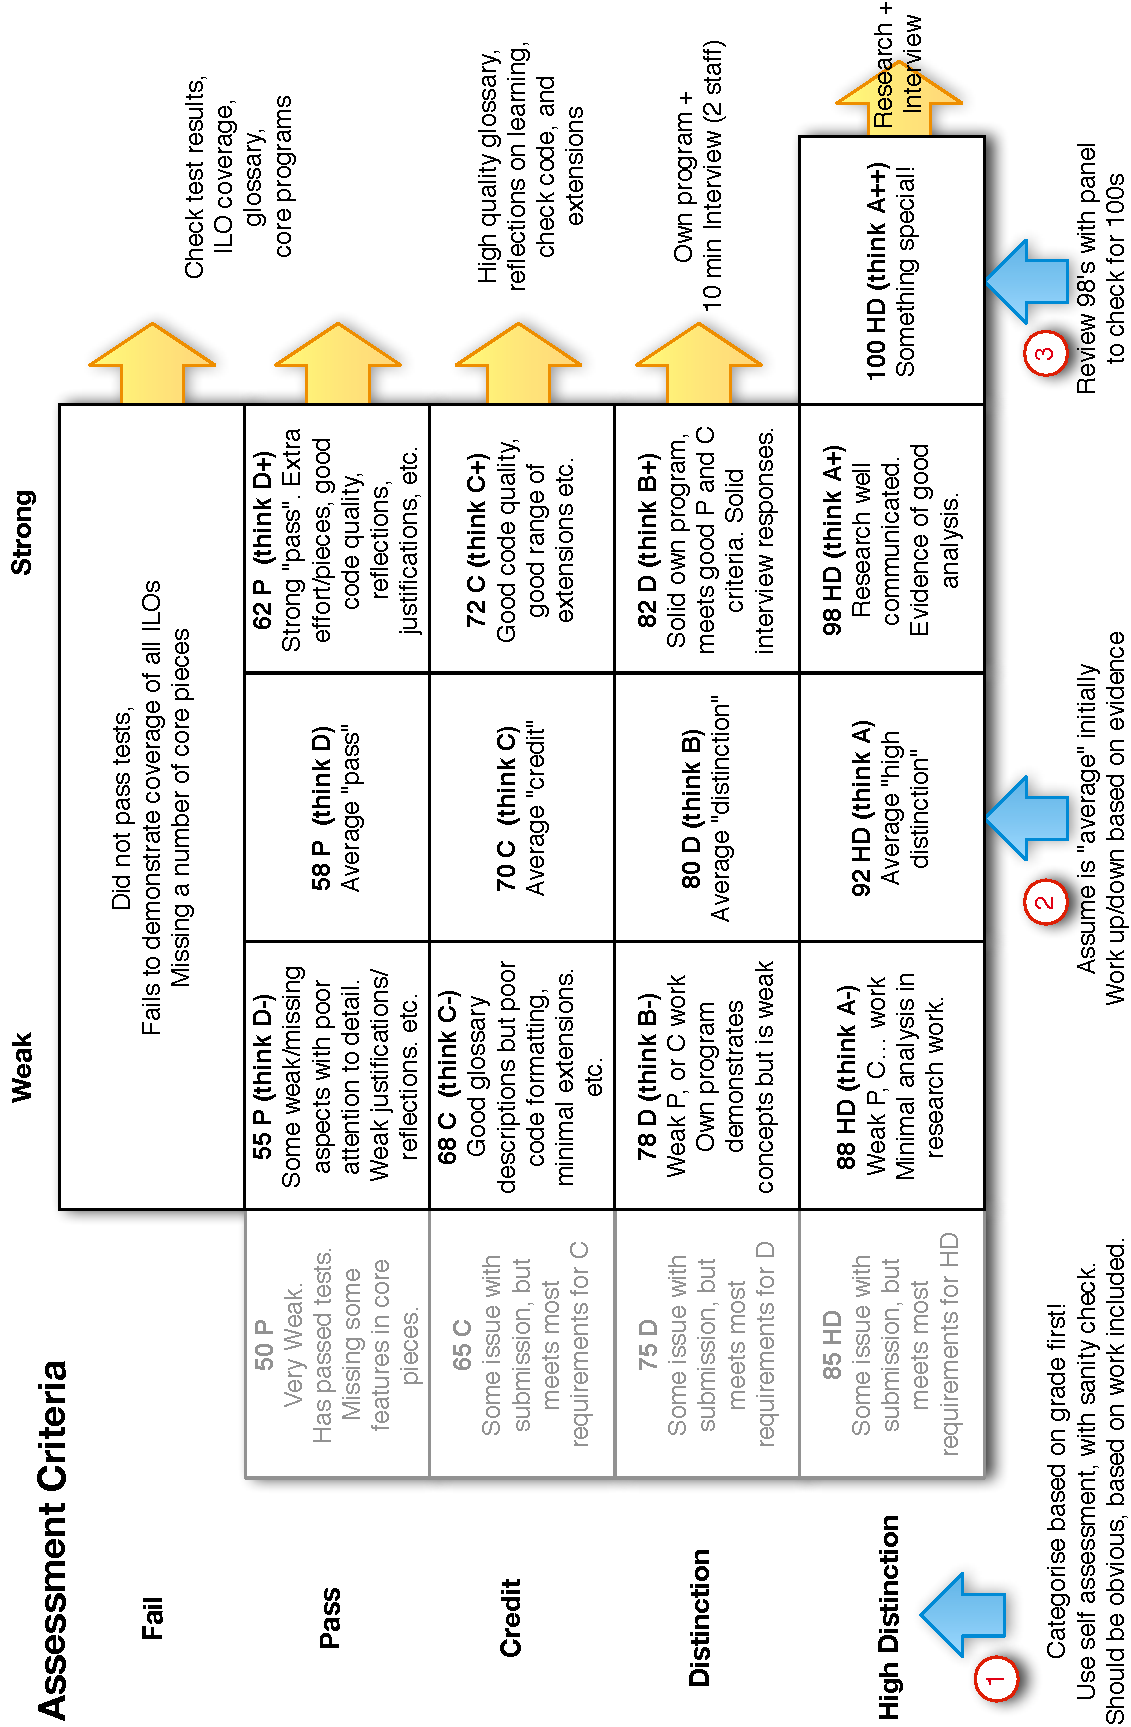
\includegraphics[width=0.98\textwidth]{AssessmentProcess}
	\caption{An overview of the assessment process used to explain the criteria to students.}
	\label{fig:assessment_process}
\end{figure}

The clearly distinct criteria for each grade made determining portfolio grades a simple task. Pass criteria required students to have satisfactorily completed the hurdle tests, Credit required a good quality glossary and all work to be signed off, Distinction the custom project, and High Distinction the research report. 

For each of the grades the quality of the distinguishing artefact needed to be checked against the expected standard. In the final portfolio assessment this task was greatly simplified due to the requirement for students to engage in the formative feedback process for Credit and higher grades. This meant that student work had already been checked by teaching staff, typically a number of time, before their portfolios are even submitted. Any issues should have been identified, and corrected, before the final summative assessment.

Students aiming for the Distinction and High Distinction grades were all interviewed. Each interview lasted around ten minutes, and was conducted by multiple teaching staff. In the interviews students were asked to discuss their custom project and research report. The portfolio was used to guide the discussion, with screen shots and print outs of the code being referred to. Overall the experience was very positive and provided teaching staff with an opportunity to engage with the students who had achieved the most in the unit.

% subsection assessing_student_portfolios (end)

\subsection{Introductory Programming in Summary} % (fold)
\label{sub:intro_summary}

This section has demonstrated the application of the model presented in \cref{cha:approach}, with the resulting unit encapsulating all of the principles from \cref{cha:guiding_principles}. The introductory programming unit was centred around its intended learning outcomes, and the central role of the learning in constructing their own knowledge. The assessment criteria rewarded students for demonstrating a depth of knowledge, pushing students to strive for a relational level of understanding. Teaching and learning activities were developed to support the constructive nature of the unit, and to provide students with a suitable challenge. All of which was supported throughout the delivery of the unit. The final assessment used the assessment criteria to quickly and efficiently determine student grade outcomes from the portfolios they submitted. 

\cref{cha:evaluation} and \cref{cha:discussion} provide further discussion of the results from delivering this unit.

% subsection summary (end)

% section introductory_programming (end)
\clearpage
\section{Object Oriented Programming} % (fold)
\label{sec:object_oriented_programming}

The second programming unit in this sequence was designed to take students who had completed the introductory programming unit, and to introduce them to the object oriented programming paradigm. This provides a second example of the implementation of the model from \cref{cha:approach}. However, as much of the application is similar to the introductory programming unit, this section will briefly discuss differences in the approach taken.

As with the introductory programming unit, the following section outline the definition of the intended learning outcomes, construction of the assessment criteria, development of the teaching and learning activities, delivery of the unit, and finally details on the assessment of the students' portfolios.

\subsection{Defining Intended Learning Outcomes} % (fold)
\label{sub:oop_defining_intended_learning_outcomes}

The intended learning outcomes for the object oriented programming unit were:
\begin{enumerate}[noitemsep,nolistsep]
	\item Explain the principles of the object oriented programming paradigm specifically including abstraction, encapsulation, inheritance and polymorphism, and explain how these principles are used to create object oriented programs.
	\item Design, develop, test, and debug object oriented programs, using an integrated development environment.
	\item Select and use appropriate collection classes, from the language's class library, to manage collections of multiple objects.
	\item Construct appropriate diagrams and textual descriptions to communicate the static structure and dynamic behaviour of an object oriented solution.
	\item Apply accepted good practices related to the construction of object oriented programs.
\end{enumerate}

Students learnt about the core principles of the object oriented programming paradigm, and how these can be used to create programs. They developed programs using an integrated development environment, which included the use of unit testing tools. Students were introduced communicating object oriented designs using the Unified Modelling Language \cite{Fowler:2004} with both class diagrams and sequence diagrams being used. Design patterns and heuristics were used to provide students with a means of evaluating the quality of their designs. As with the introductory programming unit, students used a iterative development process. 

% subsection defining_intended_learning_outcomes (end)

\subsection{Constructing Assessment Criteria} % (fold)
\label{sub:oop_constructing_assessment_criteria}

The assessment criteria from the introductory programming unit were used. These did not need adjustment as each grade was identified in a topic neutral manner. For example, for a Distinction students needed to demonstrate the \emph{application} of the unit's concepts to the creation of a program of their own design. This statement works equally well for object oriented programming paradigm as it did for procedural programming paradigm.

% subsection constructing_assessment_criteria (end)

\subsection{Developing Teaching and Learning Activities} % (fold)
\label{sub:oop_developing_teaching_and_learning_activities}

The Beyond Bullet Point approach to delivering unit concepts was applied to the presentations in this unit in the same manner as it had been applied to the introductory programming unit. The remaining lecture time, however, was used to carry out role-plays rather than demonstrate the implementation of these concepts in code.

Object oriented programming centres on the concepts of objects interacting to achieve system goals. The object oriented programming unit followed the lead of introductory programming in relegating language to a secondary role. Given that the introductory programming unit had taught students to learn syntax on their own, this unit required them to take further responsibility for learning the language and applying the concepts themselves.

Students were eased into this process, with the laboratory classes in the first week including both laboratory tasks and core tasks. After this point, however, each weeks laboratory class only contained core tasks. Laboratory classes consisted of group discussions, and enabled teaching staff to provide more in-depth feedback on students progress.

As the object oriented paradigm is best suited to developing larger solutions, the unit was divided into the development of a number of case studies. The two case studies were used to help students in both the first and second half of the unit, resulting in students developing four programs of reasonable size and complexity. In each half of the unit, one of the case studies was provided with extensive guidance. This replaced the laboratory tasks from introductory programming, but was not directly walked through in class. The second case study required the application of the same principles, but with less guidance. UML diagrams were provided to explain the design of this case study, with each iteration building a relevant part of the overall program. As the iterations progressed the details of the design were reduced, with students being required to design and implement the later iterations.

The case study from the first half of the unit developed students ability to implement basic object oriented features. \fref{fig:monopoly} shows an example UML class diagram from the last iteration of this first case. In addition to learning the required aspects of the programming language, this case study introduced students to the Model View Controller (MVC) pattern. In core tasks students developed a command line interface to the program, with extension tasks adding a second graphical interface and thereby demonstrating the benefit of the MVC approach.

\begin{figure}[htbp]
	\centering
	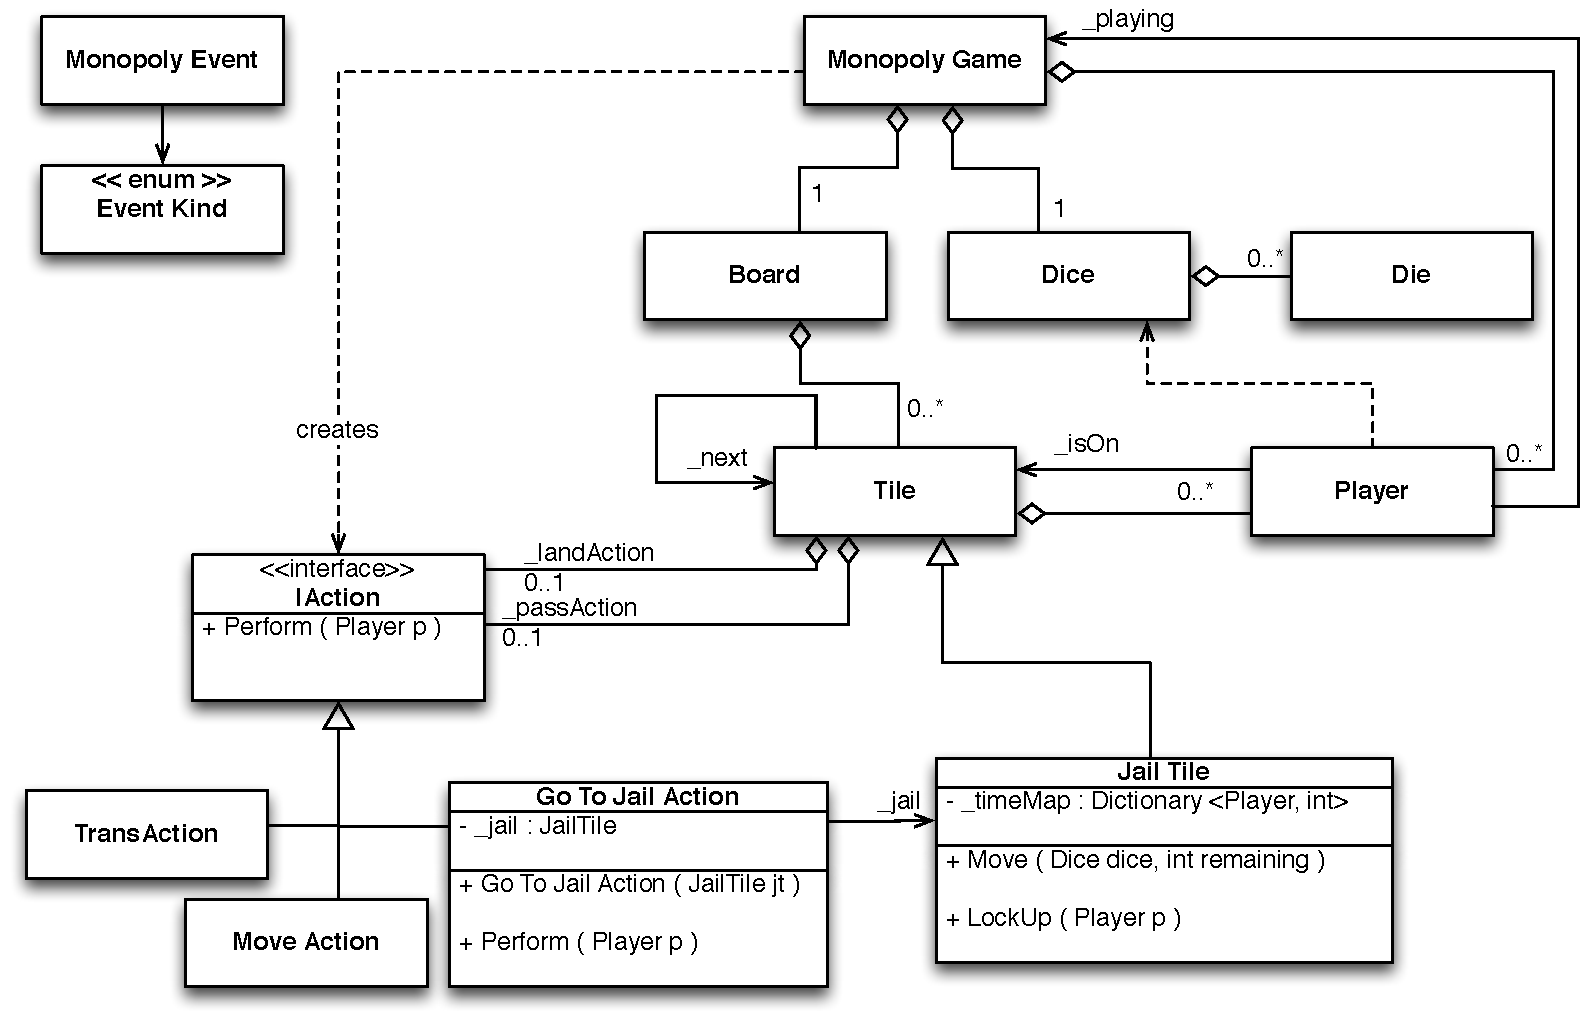
\includegraphics[width=\textwidth]{Monopoly}
	\caption{An example UML class diagram from the case studies in the object oriented programming unit..}
	\label{fig:monopoly}
\end{figure}

In the second half of the unit students took greater responsibility for the design of the program. The case study had students develop a text based adventure game, which enabled the use of the Composite and Command patterns \cite{Gamma:2001}. This program was developed over a number of iterations, with each having students implement a range of unit tests to check object functionality. As with the design aspects, the specification of the tests reduced over time with students taking full responsibility for designing the unit tests by the end of the case study.

\subsubsection{Choosing an Object Oriented Programming Language} % (fold)
\label{ssub:choosing_an_object_oriented_programming_language}

As students took an even greater responsibility for learning the language in this unit, the choice of which language to use had much greater flexibility. The choice of language was guided by the following criteria:

\begin{itemize}[noitemsep,nolistsep]
	\item Required a contemporary integrated development environment.
	\item Must support the object oriented programming paradigm.
	\item Must have unit testing tools.
\end{itemize}

Multiple languages were considered and four languages were selected: being C\#, C++, Java and Objective-C. Each of these languages had a C-style syntax, helping ease students into the new paradigm. C\#, Java and Objective-C had similar support for object oriented programming principles, with C++ being sufficient but requiring some extra attention to syntax to achieve the same outcomes. C\#, C++ and Java are statically typed, while Objective-C is dynamically typed. All had modern IDEs, and support for unit testing tools.

Unlike introductory programming, in object oriented programming students selected one language and used this throughout the unit. This forced lectures to focus more clearly on the concepts, while allowing students to focus on a language they saw as relevant to their future careers. At the same time, this also allowed comparison between different languages. The difference between static and dynamic typing were discussed in class, and demonstrated. Different approaches to memory management were also discussed, manual memory management was discussed in relation to C++, reference counting for Objective-C, and garbage collection for C\# and Java. 

Once again, the different languages helped strengthen the overall approach. This unit focused on object oriented programming, not on the specifics of a single language. The aim was not to develop a depth in \emph{one} programming language, but for students to learn the principles that underlie \emph{all} object oriented programming languages. Using multiple languages concurrently helped draw attention to this, and forced teaching staff to communicate at the concept level. 

% subsubsection choosing_an_object_oriented_programming_language (end)

% subsection developing_teaching_and_learning_activities (end)

\subsection{Assessing Student Portfolios} % (fold)
\label{sub:oop_assessing_student_portfolios}

As the assessment criteria were the same, the process of assessing student portfolios was the same as outlined for introductory programming. To pass, students had to satisfactorily complete two hurdle tests and demonstrate sufficient progress with the four case studies. Credit required a glossary that clearly documented the object oriented programming principles, and how they applied to programs the student had created. Distinction required a custom project that demonstrated the application of the object oriented programming principles, while High Distinction involved a research report.

% subsection assessing_student_portfolios (end)

% \subsection{Object Oriented Programming in Summary} % (fold)
% \label{sub:object_oriented_programming_in_summary}

% The object oriented programming unit presented here demonstrates a second application of the model presented in \cref{cha:approach}. As with the introductory programming unit, with the resulting unit encapsulated all of the principles from \cref{cha:guiding_principles}. The differences between the two units presented indicate the general applicability of the model.

% subsection object_oriented_programming_in_summary (end)

% subsection object_oriented_programming (end)

\section{Summary} % (fold)
\label{sec:ca_intro_summary}

This chapter provided two example implementations of the model described in \cref{cha:approach}. In each case the unit was developed and delivered using the processes discussed in \cref{cha:approach}, and was guided by the principles from \cref{cha:guiding_principles}. The described units have been delivery successfully across a number of teaching periods, and \cref{cha:evaluation} reports on the evaluation of these units while \cref{cha:discussion} discusses the relative importance of the various aspects of the approach overall.

In the following chapter, \cref{cha:supporting}, we describe the teaching and learning resources that supported the delivery of these units.

% section summary (end)

% chapter constructively_aligned_introductory_programming_curriculum (end)